
\chapter{مقدمه}

امروزه استفاده از تجهیزات هوشمند روز به روز در حال افزایش است و دستگاه‌هایی که قابلیت پردازش داده و ارتباط به سایر ادوات را دارند بیشتر مورد اقبال قرار می‌گیرند. ساعت‌های مچی نیز به عنوان دستگاه‌هایی که ارتباط نزدیکی با انسان دارند مورد استقبال محققان و طراحان قرار گرفتند. از این رو طراحی و ساخت ساعت هوشمند موضوعی است که برای این پژوهش انتخاب شده است.

پروژه‌ی پیش رو درباره‌ی طراحی و ساخت یک ساعت هوشمند است که توانایی‌های اکثر ساعت‌های هوشمند موجود در بازار را دارد. این توانایی‌ها شامل موارد ذیل است:
\begin{enumerate}
	\item نمایش ساعت و تاریخ
	\item ارتباط با تلفن‌همراه
	\item پخش صدا
	\item ایجاد لرزش
	\item فعال کردن آلارم در زمان مشخص
	\item شارژ کردن باتری و مدیریت توان
	\item تعامل با کاربر
	\item نمایش میزان ضربان قلب \label{item:hr}
	\item نمایش میزان سطح اکسیژن خون \label{item:spo2}
	\item شمارش تعداد گام‌های طی شده \label{item:pedo}
	\item روشن شدن صفحه نمایش در صورت بالا آمدن دست \label{item:screen}
\end{enumerate}

در راستای تحقق این اهداف، نیاز به دو بخش جداگانه وجود دارد. یک دستگاه که همان ساعت است، و دیگری تلفن‌همراه. موارد \ref{item:hr} تا \ref{item:screen} جزو کلیدی‌ترین قابلیت‌های این سیستم هستند و نیاز به پردازش داده دارند. پردازش داده‌های حرکتی که برای موارد \ref{item:pedo} و \ref{item:screen} مورد نیاز است شامل فیلتر کردن داده‌های حسگر حرکتی و سپس تصمیم گیری بر اساس آن‌ها است. این پردازش‌ها در سطح ریزپردازنده قابل پیاده‌سازی است. از این رو خود ساعت توانایی انجام این وظایف را دارد. موارد \ref{item:hr} و \ref{item:spo2} نیاز به پردازش داده‌های حسگر سلامت دارند. این داده‌ها ابتدا باید از فیلترهای مختلفی عبور کنند سپس با اعمال الگوریتم‌هایی، ضربان قلب و سطح اکسیژن خون به دست آید. از آنجا که این پردازش‌ها به منابع سخت‌افزاری بیشتری نیاز دارند، در سطح ریزپردازنده قابل اجرا نیستند. از این رو این پردازش‌ها به تلفن‌همراه منتقل می‌شود.

با توجه نیازسنجی‌های فوق، می‌توان بلوک دیاگرام سیستم و سخت‌افزار در حلقه\footnote{\lr{Hardware in the loop}}
را به صورت شکل \ref{fig:main-block} نشان داد.
\newpage
\begin{figure}[h!]
	\centering
	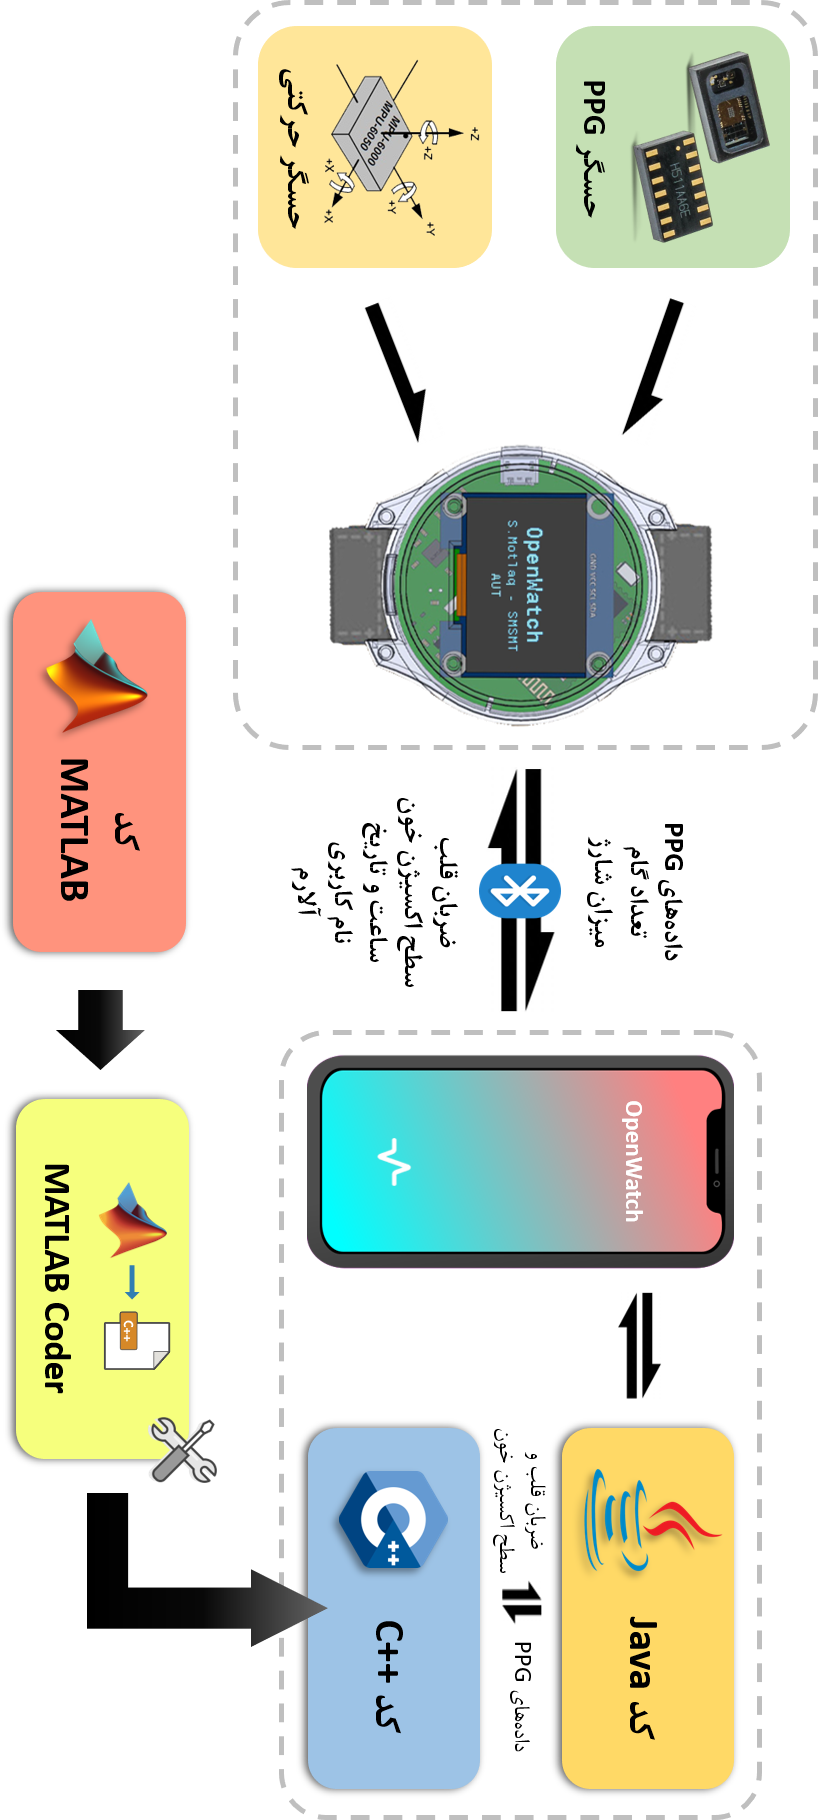
\includegraphics[width=0.64\textwidth]{main_block}
	\caption{شماتیک کلی پروژه و گذر داده}
	\label{fig:main-block}
\end{figure}
\newpage

همانطور که در شکل \ref{fig:main-block} دیده می‌شود، دو قسمت عمده وجود دارد. یکی ساعت هوشمند و دیگری تلفن‌همراه. در نیمه‌ی سمت چپ ساعت قرار داد. ورودی‌های این بخش داده‌های حرکتی و داده‌های حسگر
\lr{PPG}\footnote{\lr{Photoplethysmogram} - تغییرحجم‌سنجی نوری}
است.

داده‌های حسگر حرکتی داخل خود به کمک فیلتر کالمن فیلتر شده و از روی آن‌ها وضعیت تعداد گام و چرخش دست مشخص می‌شود. داده‌های \lr{PPG} اما به دلیل حجم بالای پردازش بر بستر بلوتوث به تلفن‌همراه ارسال می‌شود.

در نیمه‌ی سمت راست تلفن‌همراه داده‌ها را از ساعت دریافت می‌کند. یک برنامه به زبان جاوا\footnote{\lr{Java} - یک زبان برنامه‌نویسی} وجود دارد که همان برنامه‌ی اصلی اندروید است. این برنامه داده‌های حسگر را دریافت می‌کند و پس از اعتبارسنجی، آن را از طریق مجموعه ابزار
\lr{NDK}\footnote{\lr{Native Development Kit} - ابزاری که اجازه می‌دهد برنامه‌های \lr{C/C++} در سیستم عامل اندروید اجرا شوند.}
به بلوک بعدی می‌دهد.

بلوک بعدی یک کد به زبان \lr{C++} است. این کد وظیفه‌ی اصلی پردازش داده‌ها را برعهده دارد. تمام الگوریتم‌های پردازشی و فیلترهای متنوع در این کد جای دارند. خروجی این کد همان داده‌های موردنیاز یعنی نرخ ضربان قلب و سطح اکسیژن خون است. این داده‌ها مجددا از طریق کد جاوا و بستر بلوتوث به ساعت ارسال می‌شود که روی صفحه نمایش آن نمایش داده شود.

 \begin{figure}[h]
	\centering
	\begin{subfigure}{0.24\textwidth}
		\centering
		
\includegraphics[width=\linewidth]{matlab}
		\caption{\lr{MATLAB}}
		%\label{fig:stm32_image}
	\end{subfigure}
	\begin{subfigure}{0.24\textwidth}
		\centering
		
\includegraphics[width=\linewidth]{android}
		\caption{\lr{Android}}
		%\label{fig:stm32_real}
	\end{subfigure}
	\begin{subfigure}{0.24\textwidth}
		\centering
		
\includegraphics[width=0.7\linewidth]{stm32}
		\caption{\lr{STM32}}
		%\label{fig:stm32_image}
	\end{subfigure}
	\begin{subfigure}{0.24\textwidth}
		\centering
		
\includegraphics[width=0.9\linewidth]{arm}
		\caption{\lr{ARM}}
		%\label{fig:stm32_image}
	\end{subfigure}
	\caption{برخی ابزارها و فناوری‌های استفاده شده در این پروژه}
	\label{fig:techs}
\end{figure}

نکته‌ی حائز اهمیت آن است که الگوریتم‌های پردازشی و فیلترهای مورد بحث، در نرم‌افزار \lr{MATLAB} طراحی و پیاده‌سازی شده‌اند. از آنجا که اندروید توانایی اجرای کد \lr{MATLAB} را ندارد، از ابزاری به نام \lr{MATLAB Coder} استفاده شد. این ابزار برنامه‌ای را که به زبان \lr{MATLAB} نوشته شده است به زبان‌های سطح پایین‌تر مانند \lr{C} و \lr{C++} تبدیل می‌کند. از طرفی اندروید به واسطه‌ی ابزار \lr{NDK} توانایی اجرای برنامه‌های \lr{C/C++} را دارد. بنابراین معماری نرم‌افزار تلفن‌همراه به سمتی رفت که برنامه‌ی نوشته شده در \lr{MATLAB} را اینگونه اجرا کند.

قسمت‌های مربوط به الگوریتم‌های پردازش سیگنال \lr{PPG} و فیلترهای موردنیاز و همچنین برنامه‌نویسی تلفن‌همراه توسط همکار عزیزم در این پروژه، آقای سید محمد صالح میرزاطباطبایی به انجام رسیده است. توضیحات مربوطه به بخش‌های فوق در پایان‌نامه‌ی ایشان قابل دسترس است.

با توجه به نیازهایی که در ابتدای مقدمه گفته شد، یک سخت‌افزار کامل از صفر طراحی و ساخته شد. این سخت‌افزار در فصل \nameref{chap:hardware} مورد بحث قرار می‌گیرد. بدیهی است که هر سخت‌افزار نیاز به جعبه و ملاحظات فیزیکی دارد. از این رو یک بدنه برای آن طراحی و ساخته شد. جزئیات این بخش در فصل \nameref{chap:mechanical} بررسی خواهد شد. در ادامه این سخت‌افزار و ریزپردازنده نیاز به یک برنامه یا نرم‌افزار دارد که بتواند وظایف خود و پردازش‌های موردنظر را انجام دهد. پس یک برنامه به زبان \lr{C} نوشته شد که در فصل \nameref{chap:firmware} به شرح مفصل آن پرداخته شده است.

در سمت ساعت هوشمند، یک ریزپردازنده با نام \lr{STTM32F030} تعبیه شده است. این ریزپردازنده محصول شرکت \lr{ST} است. این شرکت علاوه بر تولید محصولات سخت‌افزاری و ریزپردازنده، محصولات نرم‌افزاری و ابزارهای مرتبط نیز ساخته است. یکی از این ابزارها نرم‌افزار \lr{CubeMX} است. این نرم‌افزار کار برنامه‌نویسی برای ریزپردازنده را بسیار تسریع می‌کند. بدون این ابزار مجبور به خواندن مستقیم از حافظه و نوشتن مستقیم در آن هستیم. این کار در اصطلاح فنی «برنامه‌نویسی رجیستری» نام دارد که کار دشواری است. اما به کمک ابزار \lr{CubeMX} و کتابخانه‌هایی که وجود دارد این کار تسهیل می‌شود. جزئیات بیشتر این ابزار و استفاده از آن در فصول آتی مطرح شده است.

برای فیلتر کردن داده‌های حسگر حرکتی، از فیلتر کالمن استفاده شده است. این فیلتر بهینه‌ترین فیلتر از لحاظ کمینه کردن ماتریس کوواریانس خطا است. از آنجا که معادلات حرکت معادلات دینامیکی هستند، استفاده از فیلتر کالمن گزینه‌ی مناسبی است. اما پیاده‌سازی این فیلتر نیازمند محاسبات ماتریسی و حجم پردازش بالا است. پس برای آنکه بتوان آن را در ریزپردازنده با قدرت محدود استفاده کرد باید از فنون و شیوه‌هایی بهره برد. این موارد در فصل \nameref{chap:firmware} و بخش \nameref{sec:kal} بسط داده شده‌اند.

در نهایت نیز جمع‌بندی و دورنمای کار در بخش \nameref{sec:result} آورده شده‌است.